%% evenend-ja.tex：evenendパッケージのマニュアル
%% LuaLaTeXで2回組む．見本（evenend-sample.pdf，evenend-sample-column.pdf）を
%% 先に組んでおくこと
\documentclass[paper=a4,fontsize=10pt]{jlreq}
\usepackage{graphicx}
\usepackage{hyperref}
\hypersetup{hidelinks,pdftitle={evenendパッケージ},pdfauthor={Yuwsuke Kieda}}

\newcommand\cs[1]{\texttt{\textbackslash #1}}
\newcommand\opt[1]{\texttt{#1}}
\newcommand\pkg[1]{\textsf{#1}}

\title{\pkg{evenend}パッケージ\\[.5\baselineskip]
  \large 多段組の最終ページで各段の下端を揃える}
\author{Yuwsuke Kieda}
\date{v20260925.0}

\begin{document}
\maketitle

\section{概要}

\pkg{evenend}は，LaTeXの段組（\cs{twocolumn}）で組んだ文書の最終ページについて，
各段の下端を揃えるLuaLaTeX用のパッケージである．目的は\pkg{flushend}（\pkg{sttools}）と
同じだが，次のものも扱う．
\begin{itemize}
  \item 3段以上の段組（\opt{columns=3}など）
  \item 段内フロート（最右段に載ったものを含む）と段抜きフロート（上端，
    \pkg{stfloats}による下端）
  \item 最終ページの脚注．参照位置が別の段へ移れば脚注も移し，版面の下端または
    段（カラム）の下端に置く．段をまたいで分割された脚注は1つにまとめ直す
\end{itemize}

行数によっては最右段だけが短くなる．たとえば2段で31行なら，16行と15行になる．
それ以外の段の下端は揃う．

図\ref{fig:sample}に，均した最終ページの例を示す．左は脚注を版面の下端に置いた場合
（\opt{footnote=page}，既定），右は各段の下端に置いた場合（\opt{footnote=column}）である．
どちらも，脚注は参照位置のある段に入っている．

\begin{figure}[tb]
  \centering
  \fbox{\includegraphics[page=2,width=.4\linewidth]{evenend-sample.pdf}}\hspace{2\zw}%
  \fbox{\includegraphics[page=2,width=.4\linewidth]{evenend-sample-column.pdf}}
  \caption{均した最終ページ．左は\opt{footnote=page}，右は\opt{footnote=column}
    （\texttt{evenend-sample.tex}，\texttt{evenend-sample-column.tex}）}
  \label{fig:sample}
\end{figure}

\section{動作要件}

\begin{itemize}
  \item LuaLaTeX（LaTeX 2023-06-01以降）．pLaTeX，upLaTeX，pdfLaTeXでは使えない．
  \item LaTeX標準の段組（クラスオプション\opt{twocolumn}または\cs{twocolumn}）．
    \pkg{multicol}の\texttt{multicols}環境は対象外である．
  \item \pkg{jlreq}，\pkg{ltjsclasses}，\pkg{article}で動作を確かめている（横組のみ）．
\end{itemize}

\section{インストール}

\texttt{evenend.sty}と\texttt{evenend.lua}を，TEXMFツリーの
\texttt{tex/lualatex/evenend/}に置く．配布物のディレクトリをそのままTEXMFHOMEに
してもよい．
\begin{verbatim}
export TEXMFHOME=/path/to/texmf-evenend
\end{verbatim}

\section{使い方}

プリアンブルで読み込むだけで，文書末（\verb|\end{document}|）と\cs{onecolumn}の直前の
ページが揃う．
\begin{verbatim}
\documentclass[twocolumn]{jlreq}
\usepackage[footnote=column]{evenend}
\end{verbatim}

\subsection{オプション}

\begin{center}
  \begin{tabular}{llll}
    \hline
    キー & 値 & 既定 & 意味 \\
    \hline
    \opt{columns} & 整数 & \opt{2} & 段数（読み込み時のみ） \\
    \opt{footnote} & \opt{page}／\opt{column} & \opt{page} & 最終ページの脚注の置き場所 \\
    \opt{onecolumn} & 真偽 & \opt{true} & \cs{onecolumn}の直前のページも揃える \\
    \opt{enable} & 真偽 & \opt{true} & 文書末のページを揃える \\
    \opt{debug} & 真偽 & \opt{false} & 段ごとの高さなどをログに書く \\
    \hline
  \end{tabular}
\end{center}

\begin{description}
  \item[\opt{columns}] 段数．3以上にすると，段幅を
    $(\cs{textwidth}-(N-1)\cs{columnsep})/N$にする（$N$は段数）．
    読み込み時にしか指定できない．
  \item[\opt{footnote}] \opt{page}では，本文を揃えた段の下を空け，脚注を版面の下端に置く．
    \opt{column}では，脚注を含めた各段の下端が揃う．どちらの場合も，脚注は参照位置の
    ある段に入る．
  \item[\opt{onecolumn}] \cs{onecolumn}で段組を終えるときも，その直前のページを揃える．
  \item[\opt{enable}] 偽にすると，文書末のページを揃えない（\cs{raggedend}と同じ）．
  \item[\opt{debug}] 揃えた段の高さ，段ごとの本文・フロート・脚注の高さをログに書く．
\end{description}

\opt{columns}以外のキーは，文書中でも\cs{evenendsetup}で変えられる．

\subsection{命令}

\begin{description}
  \item[\cs{evenend}，\cs{raggedend}] 文書末のページを揃えるかどうかを切り替える．
  \item[\cs{evenendclearpage}] いまのページを揃えてから改ページする．章末などに使う．
  \item[\cs{evenendsetup}\texttt{\{}\textit{キー}\texttt{=}\textit{値}\texttt{\}}]
    オプションを変える．
\end{description}

\section{揃え方}

\subsection{段の高さ}

最終ページの本文を，入り切る最小の段の高さで各段に分け直す．このとき，段内フロートと，
段に入る脚注の高さを差し引く．残りを最右段に入れるので，行数が段数で割り切れなければ，
最右段だけが短くなる．

各段では「見かけの下端」を揃える．
\begin{itemize}
  \item 本文で終わる段：最終行の字面の下端（ベースライン＋深さ）
  \item 下のフロートで終わる段：フロートの下端
  \item 段下端の脚注で終わる段（\opt{footnote=column}）：脚注の最終行の字面の下端
\end{itemize}
最後の要素が垂直の箱で，中身が箱の下端からはみ出している場合（中身をグルーで下へずらした
箱など）は，はみ出した位置を下端とみなす．

本文だけの満杯の段があれば，その段を基準にする．フロートのある段は，フロートまわりの
グルーの伸び縮みで合わせる．こうすると，行の位置が段の間で揃う．段の高さに届かない段
（行の足りない最右段や，版面下端の脚注に押された段）は，グルーを伸ばさずに下を空ける．

\subsection{フロート}

\begin{itemize}
  \item 段内フロートは，もとの段に残す．上のフロートは段の上端に，下のフロートは段の
    下端に付ける．
  \item 段抜きフロートは，LaTeX本来の処理（\cs{@combinedblfloats}）がこれまでどおり
    配置する．\pkg{stfloats}による段抜きの下のフロートは，揃えた段の下に来る．
  \item 最終ページにフロートだけの段（フロート段）がある場合は揃えず，警告を出す．
\end{itemize}

\subsection{脚注}

最終ページの脚注は，本文中の参照位置が入った段へ移す．TeXが段をまたいで分割した脚注は，
1つにまとめ直す．参照位置が最終ページにない脚注（前のページから送られてきたもの）は，
もとの段に残す．

\begin{itemize}
  \item \opt{footnote=page}：脚注は版面の下端に置く．本文の段の下との間は空く．
  \item \opt{footnote=column}：脚注は各段の本文の下に置き，脚注の最終行の字面の下端を，
    他の段の下端に揃える．
\end{itemize}

\section{仕組み}

\begin{enumerate}
  \item 各段を出力するとき（\cs{@makecol}の直前），段の生の材料（\cs{box255}），改段位置で
    捨てられるグルー類，脚注（\cs{box}\cs{footins}），段内フロートの複製を，Lua側に
    とっておく．
  \item 脚注には番号をLuaTeXの属性として付け，本文中の参照位置には同じ番号の印
    （\cs{vadjust}で行の直後に置くwhatsit）を置く．
  \item 最終ページの最後の段が，\cs{clearpage}の強制改段で出力されるとき，そのページの全段の
    材料を1本の垂直リストにつなぎ直す．そのうえで，入り切る最小の段の高さを探して，
    \cs{vsplit}で分け直す．
  \item 段を組み直し，段抜きフロートを加えて出力する．
\end{enumerate}

最終ページ以外の組版は，このパッケージを読み込まない場合と変わらない．

段組の出力ルーチン\cs{@outputdblcol}は，このパッケージが置き換える．3段以上の段組も
ここで扱う．

\section{他のパッケージとの併用}

\begin{itemize}
  \item \pkg{hyperref}：併用できる．
  \item \pkg{stfloats}：併用できる．段抜きのフロートを下に置いても揃う．
  \item \pkg{gyoudori}：併用できる．行ドリしたフロートも，行送りの位置に揃う．
  \item \pkg{flushend}，\pkg{balance}など\cs{@outputdblcol}を置き換えるパッケージ：
    併用できない．
\end{itemize}

\section{制限事項}

\begin{itemize}
  \item 最終ページ内の強制改段（\cs{newpage}など）は無視して詰め直す．
  \item 脚注は段をまたいで分割しない．
  \item 段内フロートはもとの段に残る．参照位置との前後関係は保証しない．
  \item \cs{marginpar}の左右は計算し直さない．
  \item 縦組には対応していない．
\end{itemize}

\section{配布物}

\begin{description}
  \item[\texttt{tex/lualatex/evenend/}] \texttt{evenend.sty}，\texttt{evenend.lua}
  \item[\texttt{doc/lualatex/evenend/}] このマニュアル（\texttt{evenend-ja.tex}）と
    見本（\texttt{evenend-sample.tex}，\texttt{evenend-sample-column.tex}）
  \item[\texttt{LICENSE}] ライセンス（MIT）
  \item[\texttt{test/}] テスト文書と補助スクリプト（\texttt{run.sh}，
    \texttt{colbottoms.py}，\texttt{fuzz.sh}）
\end{description}

このマニュアルを組むには，先に見本を組む．
\begin{verbatim}
lualatex evenend-sample.tex
lualatex evenend-sample-column.tex
lualatex evenend-ja.tex
lualatex evenend-ja.tex
\end{verbatim}

\section{バージョン表記}

バージョンは\texttt{v}\textit{年月日}\texttt{.}\textit{番号}と表す．\textit{年月日}は
変更した日（8桁），\textit{番号}はその日のうちの変更回数（0から数える）である．
たとえば\texttt{v20260925.0}は，2026年9月25日の最初の版を表す．

\section{ライセンス}

MITライセンス（配布物の\texttt{LICENSE}を参照）．

Copyright (c) 2026 Yuwsuke Kieda

\end{document}
